\chapter{Hidden Markov Map Matching}

Source: \cite{newson2009hidden}.

\section{论文动机}

\subsection{原始数据}

the raw input
data consists of vehicle \term{locations} measured by GPS, Each measured point consists of a time-stamped
latitude/longitude pair. 

The \term{roads} are also represented in the
conventional way, as a graph of nodes and edges.
The \term{nodes} are at
intersections, dead ends, and road name changes, and the edges
represent road segments between the nodes. Some \term{edges} are
directional to indicate one-way roads. Each node has an associated
latitude/longitude to indicate its location, and each edge has a
polyline (折线) of latitude/longitude pairs to represent its geometry.

\section{其他论文的方法}

平滑曲线匹配:create a (possibly smoothed) curve
from the location measurements and attempt to find matching
roads with similar geometry

\begin{example}
White et al. 
present four algorithms, starting with the simple, nearest match
scheme. 
Their second algorithm \textbf{adds orientation information to
the nearest match approach}, comparing the measured heading to
the angle of the road. Their third algorithm evolves the second
algorithm to \textbf{include connectivity constraints}, and their fourth
algorithm does \textbf{curve matching}. 

\begin{remark}
    their most sophisticated algorithm, the fourth one, was
outperformed by the simpler second algorithm.
\end{remark}
\end{example}

通过拓扑结构建模:builds up a
topologically feasible path through the road network. Matches are
determined by a similarity measure that weights errors based on
distance and orientation. The algorithm was found to perform flawlessly, even though the GPS data was collected while
\term{Selective Availability} was turned on, leading to noisier location
measurements than are available now.

模糊匹配策略:Kim and Kim look at a
way to measure \textbf{how much each GPS point belongs to any given road}, taking into account its distance from the road, the shape of
the road segment, and the continuity of the path. The measure is
used in a \textbf{fuzzy matching scheme} with learned parameters to
optimize performance.

Brakatsoulas et al. Their
algorithm uses variations of the \term{Fréchet distance} to match the
curve of the GPS trace to candidate paths in the road network.

\begin{remark}
    One potential problem with purely geometric approaches is \textbf{their
sensitivity to measurement noise and sampling rate.} 
Connecting the dots of a set of noisy measurements sampled at a
slow rate would not match well with the road geometry, especially
\textbf{direction information}.
\end{remark}

基准方法:将GPS点匹配到最近邻的路上

\begin{remark}
    result in extremely unreasonable paths involving strange U-turns, inefficient looping, and overall bizarre driving
behavior.
\end{remark}

\section{论文贡献}

\begin{itemize}
    \item maintaining a principled approach to the problem while simultaneously making the algorithm robust to location data that is both \textbf{geometrically noisy and temporally sparse}
    \item a test of our map matching algorithm where we vary the levels of noise and sparseness of the sensed location data over a 50 mile urban drive
\end{itemize}

\begin{remark}
   问题: \ref{Problem:PureHMM1} \ref{Problem:PureHMM2} 
\end{remark}

\section{论文模型-Hidden Markov Model}

The HMM models processes that involve a path through many
possible states, where some state transitions are more likely than
others and where the state measurements are uncertain.

\subsection{HMM}

\begin{figure}[h]
    \centering
    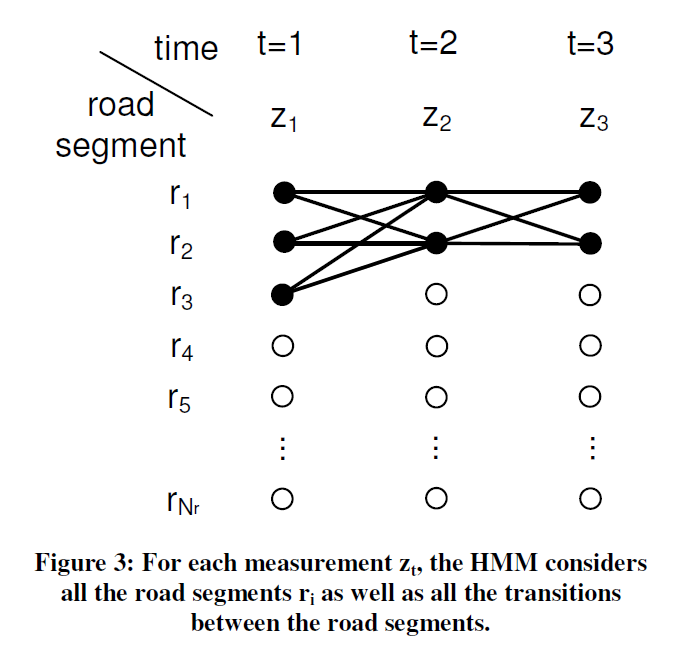
\includegraphics[scale=0.4  ]{hmm-hmm-of-observation.png}
\end{figure}

\begin{itemize}
    \item HMM状态:$ N_{r} $ individual  road  segments $ r_{i},  i=1 \ldots N_{r} $
    \item 状态的测量:每次带噪声的位置数据 $ Z_{t} $
    \item 候选路径:有很多,可能有很曲折的
    \item 目标:将每个GPS点匹配到合适的路段上
\end{itemize}

\subsection{已知在这个路段得到这个GPS点位置的概率估计}

\begin{figure}[h]
    \centering
    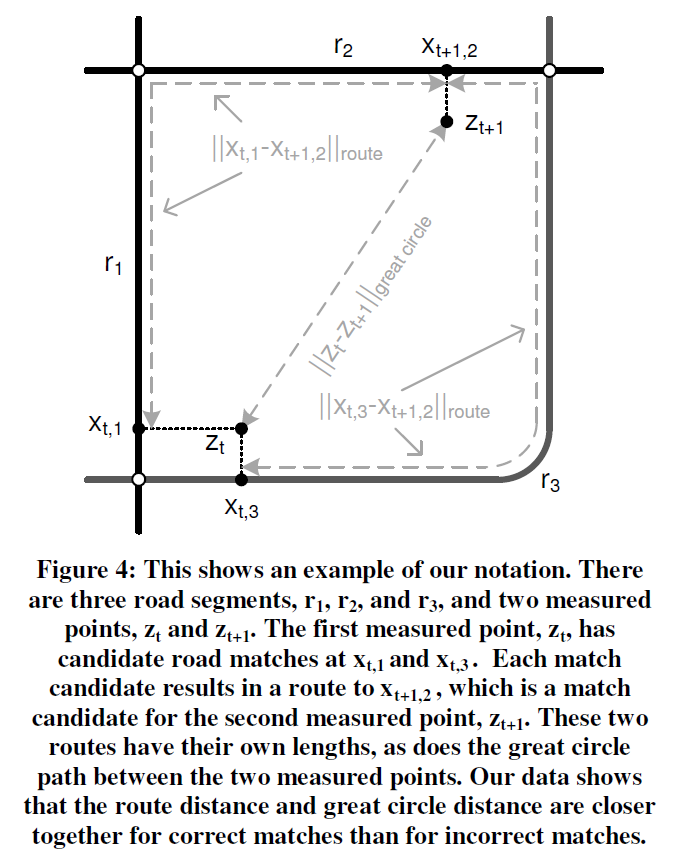
\includegraphics[scale=0.4  ]{HMM-mapping.png}
\end{figure}

对于给定的$z_{t},r_{i} $有\term{emission probability}$ x_{t, i}$. 

估计方法:
The \term{great circle distance} on the surface of the earth between the measured point and the candidate match is $ \| z_{t}- x_{t, i} \|_{great\_circle}$. For the correct match, this difference is due to GPS noise. 噪声认为是零均值的高斯噪声. 

$$ p\left(z_{t} \mid r_{i}\right)=\frac{1}{\sqrt{2 \pi} \sigma_{z}} e^{-0.5\left(\frac{\left\|z_{t}-x_{t, i}\right\|_{\text {great circle }}}{\sigma_{z}}\right)^{2}} $$

$\sigma_{z}$是GPS测量的方差(需要估计). 

对于初始状态$ \pi_{i} ,i=1 \ldots N_{r} $(指定一开始车辆在所有路段上的可能性),为了简化使用$$ \pi_{i}=p\left(z_{1} \mid r_{i}\right) $$

\subsection{转移概率}

Each measurement $ z_{t} $ has a list of possible road matches, as does the next measurement $ z_{t+1} $. 

作者认为\textbf{测量距离和大圆距离相近的状态转移才是比较好的},否则会绕路(概率下降). 

计算发现大圆距离与路径距离的差值绝对值近似于:

$$ p\left(d_{t}\right)=\frac{1}{\beta} e^{-d_{t} / \beta} $$

路径距离$ d_{t}=\left| \left\|z_{t}-z_{t+1}\right\|_{\text {great circle }}-\left\|x_{t, i^{*}}-x_{t+1, j^{*}}\right\|_{\text {route }}\right| $是动态规划(\term{Viterbi algorithm})得到的路线距离. 对于$z_t$和候选路段$r_i$,匹配出在路段上的点是$ x_{t, i} $. 

\begin{remark}
      \label{Comment:HMM-TransitionProbability}

      the transition probability
        dependence on the current and previous observations
    violates the properties of an ideal HMM

    这个度量没有考虑不同采样频率的差异性. 它依赖于当前和先前位置观测之间的距离, 受到位置测量误差的不利影响. 在高位置误差的影响下误差大 \cite{Jagadeesh2017}.
\end{remark}

\section{算法的实现}

\begin{itemize}
    \item 数据预处理的时候对于离上一个GPS点位置超过$ 2 \sigma_{z} $的点进行剔除
    \item 将离GPS位置观测值200米以外路段的观测概率设为0
    \item 对于大圆距离和路径距离超过2公里路径的观察概率设为0
    \item 对于明显超速的路径的概率设为0
    \item 当明显无法匹配的时候,移除一些点,尝试重新连接,如果仍旧无法连接,引入匹配断点
\end{itemize}

\subsection{参数估计}

估计GPS误差:
$ \sigma_{z} $ using the \term{median absolute deviation (MAD)}

$$ \sigma_{z}=1.4826 \mathrm{median}_{\mathrm{t}}\left(\left\|z_{t}-x_{t, i}\right\|_{\text {great circle }}\right) $$

the point on $ r_{i}^{*} $ (人工匹配的路段) nearest $ z_{t} $ is $ x_{t, i}^{*} $.

估计路径距离与大圆距离之间的差值:

$$ \begin{aligned} \beta=\frac{1}{\ln (2)} \operatorname{median}_{t} &\left(\mid\left\|z_{t}-z_{t+1}\right\|_{\text {great circle }}\right.\\ &\left.-\left\|x_{t, i^{*}}-x_{t+1, j} *\right\|_{\text {route }} \mid\right) \end{aligned} $$



\section{实验}

数据:真实驾车GPS数据、高斯噪声模拟数据

评价指标:reported error
  $$ \left(\mathrm{d}-+\mathrm{d}_{+}\right) / \mathrm{d}_{0} $$ 

  $d_{-}  $ =length erroneously subtracted,
  $ d_{+} $=length erroneously added



其他两种指标:

  Locations on Road. 
  \begin{remark}
      This accuracy measure
  says that the matched point should be in the
  same location as the actual vehicle. Since we
  measured the vehicle's location with inherently
  noisy GPS, we do not know its actual location.
  \end{remark}

  Road Segment.
  \begin{remark}
      This accuracy measure says
  that the matched point should be on the same
  road segment as the actual vehicle. While the
  correct road segment is easier to guess than the
  correct location, it is still ambiguous at
  intersections, where a noisy measurement could
  match to any of the roads converging at that
  point.
  \end{remark}
  
   